\documentclass[12pt]{article}
\usepackage[margin=1.27cm]{geometry}
\usepackage{setspace}
\usepackage{fontspec}
% \usepackage[T1]{fontenc}
% \usepackage[utf8]{inputenc}
\usepackage{amsmath,txfonts,amssymb,nicefrac,mathtools,pifont} %for math
\usepackage{array,tabularx,multirow,fmtcount} %for tables
\usepackage{tikz, pgfplots} %for diagram
\usepackage{multicol} %for multiple column
\usepackage{enumerate,enumitem,adjustbox} %for ordered list
\usepackage{graphicx,subcaption,wrapfig,tcolorbox} %for figure
\usepackage{xparse} %for commands & environments
\usepackage{lipsum} %miscellaneous
\usepackage{colortbl,xcolor,soul} %for default table & border

% #ANCHOR Font settings
\setmainfont{Oxygen}
\newfontfamily\banglafont[Script=Bengali]{Baloo Da 2}
\newfontfamily{\lstsansserif}{IBM Plex Mono}
\renewcommand{\normalsize}{\fontsize{11.5pt}{13pt}\selectfont}


\setlength{\arrayrulewidth}{0.35 pt}
\definecolor{border}{HTML}{A1A1AA}
\arrayrulecolor{border}


% #ANCHOR Document settings
\linespread{1.45}
\setlength\parindent{0pt}
\setlength\parskip{16pt}
\setlist[enumerate]{noitemsep}
\usetikzlibrary{shapes.geometric,decorations.pathreplacing,trees,arrows,positioning,shapes,fit,calc,decorations.markings, decorations.text}
\tikzset{every node/.append style={font=\footnotesize}}
\usepgfplotslibrary{fillbetween}
\pgfdeclarelayer{background}
\pgfsetlayers{background,main}
\pgfplotsset{compat=1.18}
\columnseprule=1pt
\everymath{\displaystyle}
% #ANCHOR Hypernation
\tolerance=1
\emergencystretch=\maxdimen
\hyphenpenalty=10000
\hbadness=10000
\newlength{\colWidth}



% #ANCHOR Colors
\definecolor{azure(colorwheel)}{rgb}{0.0, 0.5, 1.0}
\definecolor{carminepink}{rgb}{0.92, 0.3, 0.26}
\definecolor{orange}{rgb}{0.9, 0.55, 0.22}
\definecolor{violet}{rgb}{0.60, 0.45, 1}
% Syantax Highlighting Colors
\definecolor{keyword}{HTML}{D73A4A}
\definecolor{number}{HTML}{015CC5}
\definecolor{comment}{HTML}{6A737D}
\definecolor{string}{HTML}{1D825E}
\definecolor{function}{HTML}{743FD1}
\definecolor{orange}{HTML}{CF7842}
\definecolor{codeblack}{HTML}{24292F}
\definecolor{divider}{HTML}{A1A1AA}
\definecolor{border}{HTML}{D1D1D1}


% #ANCHOR Ordered & Unordered List
\setlist[itemize,1]{left=0cm, label={\textbullet}}
\setlist[itemize,2,3,4,5,6,7,8,9,10]{left=0.6cm, label={\textbullet}}
\setlist[enumerate,1]{left=0cm}
\setlist[enumerate,2,3,4,5,6,7,8,9,10]{left=0.6cm}
\setul{0.5ex}{0.125ex}



% #ANCHOR Colored Box
\let\oldul\ul
\renewcommand{\ul}[2][keyword]{\text{\setulcolor{#1}\oldul{#2}}}
\newcommand{\redbox}[1]{%
{\color{red}\fbox{\color{black}#1}}
}
\newcommand{\red}[1]{%
\textcolor{red}{#1}
}
\newcommand{\redeq}[1]{%
\text{\color{red}$#1$}
}
\newcommand{\mred}[1]{%
\textcolor{keyword}{#1}
}
\newcommand{\mredeq}[1]{%
\textcolor{keyword}{$#1$}
}
\newcommand{\blue}[1]{%
% {\color{number}#1\hspace{-0.4ex}}
\textcolor{number}{#1}
}
\newcommand{\blueeq}[1]{%
\text{\color{number}$#1$}
}
\newcommand{\cyanbox}[1]{%
{\color{teal}\fbox{\textcolor{black}{#1}}}
}
\newcommand{\cyan}[1]{%
\textcolor{teal}{#1}
}
\newcommand{\pink}[1]{%
\textcolor{magenta}{#1}
}
\newcommand{\orange}[1]{%
\textcolor{orange}{#1}
}
\newcommand{\violet}[1]{%
{\color{violet}#1}
}
\newcommand{\cyaneq}[1]{%
\text{\color{teal}$#1$}
}
\newcommand{\gray}[1]{%
\textcolor{comment}{#1}
}
\newcommand{\pinkeq}[1]{%
\text{\color{magenta}$#1$}
}
\renewcommand{\columnseprulecolor}{\color{divider}}




% #ANCHOR Tabular commands
\newcolumntype{P}[1]{>{\centering\arraybackslash}p{#1}}
\newcolumntype{M}[1]{>{\centering\arraybackslash}m{#1}}
\newcolumntype{C}{>{\centering\arraybackslash}X}
\newcommand{\rspan}[2]{\multirow{#1}{*}{#2}}
\newcommand{\thc}[1]{%
\multicolumn{1}{|c|}{\textbf{#1}}
}
\newcommand{\thcx}[1]{%
\multicolumn{1}{|C|}{\textbf{#1}}
}
\newcommand{\thl}[1]{%
\multicolumn{1}{|l|}{\textbf{#1}}
}
\newcommand{\thr}[1]{%
\multicolumn{1}{|r|}{\textbf{#1}}
}
% Adjusting arraystretch to modify vertical padding
\renewcommand{\arraystretch}{1.25}
% Adjusting tabcolsep to modify horizontal padding
\setlength{\tabcolsep}{10pt}



% #ANCHOR Math commands
\newcommand{\set}[1]{\{$#1$\}}
\newcommand{\tabs}{\ \ \ \ \ \ }
\newcommand{\tab}{\ \ \ }
\newcommand{\cmark}{\ding{51}}%
\newcommand{\xmark}{\ding{55}}%
\newcommand{\boldi}[1]{\boldsymbol{#1}}%
\newcommand{\wspace}{\ \ = \ \ }



% #ANCHOR New commands
\newcommand{\Title}[1]{%
   \begin{center}
      \textbf{\Large{#1}}
   \end{center}
}
\newcommand{\Heading}[1]{%
   \par\vspace{\dimexpr -\baselineskip + 16pt}
   {\fontsize{12pt}{13pt}\selectfont\textbf{#1}}
   \par\vspace{\dimexpr -\baselineskip + 6pt}
}
\newcommand{\BuleHeading}[1]{%
   \par\vspace{\dimexpr -\baselineskip + 16pt}
   {\fontsize{12pt}{13pt}\selectfont\textbf{\textcolor{number}{#1}}}
   \par\vspace{\dimexpr -\baselineskip + 6pt}
}
\newcommand{\CHeading}[1]{%
   \par\vspace{\dimexpr -\baselineskip + 16pt}
   \hspace{\fill}
   {\fontsize{12pt}{13pt}\selectfont\textbf{#1}}
   \hspace{\fill}
   \par\vspace{\dimexpr -\baselineskip + 6pt}
}
\newcommand{\Section}[1]{%
   \par\vspace{\dimexpr -\baselineskip + 16pt}
   \hspace{\fill}
   {\fontsize{13pt}{13pt}\selectfont\textbf{#1}}
   \hspace{\fill}
   \par\vspace{\dimexpr -\baselineskip + 6pt}
}
\newcommand{\seteqno}[1]{%
   \ \cdots \ \cdots \ \cdots \ (#1)
}
\newcommand{\eqor}{%
   \Rightarrow \ \ 
}
\newcommand{\tsub}[1]{%
\textsubscript{#1}\hspace{-0.45ex}
}
\newcommand{\tsup}[1]{%
\textsuperscript{#1}\hspace{-0.45ex}
}
\newcommand{\cbox}[2][cyan]{
\tikz\node[draw=#1,circle,inner sep=2pt,baseline=(a.base)](a){#2};
}
\newcommand{\hrline}{%
\vspace{1ex} {\color{gray}\hrule} \vspace{4ex}
}
\newcommand{\divideX}[1][divider]{{\hspace{1ex}\color{#1}{\vrule}\hspace{1ex}}}
\newcommand{\Reference}[2][Reference]{

\vspace{-0.5\baselineskip}
\begin{center}
   {\fontspec{Merriweather}\textbf{#1:} \textit{#2}} 
\end{center}
}
\newcommand{\bn}[1]{%
   {\banglafont #1}
}

\NewDocumentCommand{\Column}{O{0.49} O{1.5em} m m}{
   \setlength{\colWidth}{\linewidth-#1\linewidth-#2}
   \begin{minipage}[t]{#1\linewidth}
      \noindent
         #3
      \end{minipage}\hspace{\fill}{\color{divider}\vrule width 0.35pt}\hspace{\fill}
      \begin{minipage}[t]{\colWidth}
      \noindent
         #4
   \end{minipage}
}

\usepackage{circuitikz}
\usepackage{tikz}

\ctikzset{resistors/scale=0.65}
\ctikzset{diodes/scale=0.75}
\ctikzset{sources/scale=0.75}

\begin{document}
\Title{Operational Amplifier (Op-Amp)}

% \begin{center}
%    \begin{circuitikz}
%    \draw
%       (0, 0) node[op amp] (opamp) {}
%       (opamp.-) -- ++(-0.5,0)
%       node[left]{Inverting \ input $(v_1)$}
%       (opamp.+) -- ++(-0.5,0)
%       node[left]{Non-Inverting \ input $(v_2)$}
%       (opamp.out) -- ++(0.5,0)
%       node[right]{Output}
%       (opamp.up) -- ++(0,1)
%       node[above]{$+v_s$}
%       (opamp.down) -- ++(0,-1)
%       node[below]{$-v_s$}
%    ;\end{circuitikz}
% \end{center}


\vspace{-1.5\baselineskip}
\CHeading{Op-Amp: \cyan{Single Ended Mode}}
% Single-ended input operation results when the input signal is connected to one input with the other input connected to ground.

\begin{center}
\begin{minipage}{0.49\textwidth}
   \centering
   \begin{circuitikz}
      \draw
         (0, 0) node[op amp] (opamp) {}
         (opamp.-) -- ++(-0.5,0) to[R,l_=$R_1$,anchor=east] ++(-1.5, 0) -- ++(0,-0.5)
         to[sV, fill=white] ++(0,0) -- ++(0,-0.5)
         node[label=below:$V_{i}$]{}
         (opamp.-) to[short,*-] ++(0,1) coordinate (leftC)
         to[R=$R_f$] (leftC -| opamp.out)
         to[short,-*] (opamp.out) to [short,-o] ++(1,0)
         node[label=right:$V_{o}$]{}
         (opamp.+) -| ++(-0.5,-0.5) node[ground]{}
   ;\end{circuitikz}

   Inverting Amplifier

   \vspace{-\baselineskip}
   $$Av = -\frac{R_f}{R_1}$$
   \begin{center}
      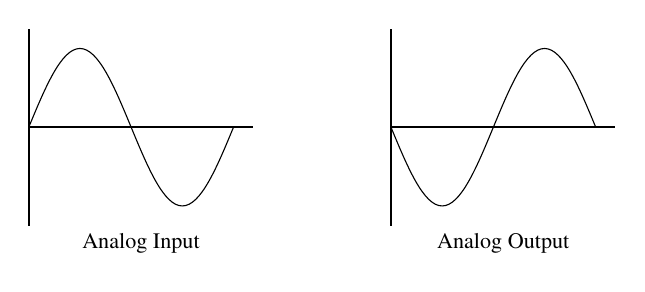
\begin{tikzpicture}
         % Coordinates
         \def\p{0.65}
         \coordinate (Origin1) at (0,0);
         \coordinate (Origin2) at (4.6,0);
         % Captions
         \draw[thick] (Origin1) -- ++(\p*4+0.25, 0)
         node[midway,below=1.2cm]{Analog Input};
         \draw[thick] (Origin2) -- ++(\p*4+0.25, 0)
         node[midway,below=1.2cm]{Analog Output};
         % Input wave
         \draw[thick] (Origin1) -- ++(0,1.25) (Origin1) -- ++(0,-1.25);
         \draw (Origin1) sin ++(\p,1) cos ++(\p,-1) sin ++(\p,-1) cos ++(\p,1);
         % Output wave
         \draw[thick] (Origin2) -- ++(0,1.25) (Origin2) -- ++(0,-1.25);
         \draw (Origin2) sin ++(\p,-1) cos ++(\p,1) sin ++(\p,1) cos ++(\p,-1);
      \end{tikzpicture}
   \end{center}

\end{minipage}{\vrule width 1pt}
\begin{minipage}{0.49\textwidth}
   \centering
   \begin{circuitikz}
      \draw
         (0, 0) node[op amp] (opamp) {}
         (opamp.-) -- ++(-0.5,0) to[R,l_=$R_1$,anchor=east]
         ++(-2, 0) node[ground]{}
         (opamp.-) to[short,*-] ++(0,1) coordinate (leftC)
         to[R=$R_f$] (leftC -| opamp.out)
         to[short,-*] (opamp.out) to [short,-o] ++(1,0)
         node[label=right:$V_{o}$]{}
         (opamp.+) -- ++(-0.3,0)
         to[sV, fill=white] ++(0,0) to[short,-o] ++(-0.7,0)
         node[label=left:$V_{i}$]{}
   ;\end{circuitikz}
   Non-Inverting Amplifier

   \vspace{-\baselineskip}
   $$Av = 1+\frac{R_f}{R_1}$$

   \vspace{1ex}
   \begin{center}
      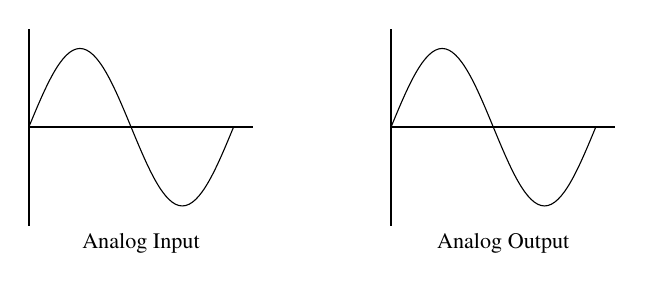
\begin{tikzpicture}
         % Coordinates
         \def\p{0.65}
         \coordinate (Origin1) at (0,0);
         \coordinate (Origin2) at (4.6,0);
         % Captions
         \draw[thick] (Origin1) -- ++(\p*4+0.25, 0)
         node[midway,below=1.2cm]{Analog Input};
         \draw[thick] (Origin2) -- ++(\p*4+0.25, 0)
         node[midway,below=1.2cm]{Analog Output};
         % Input wave
         \draw[thick] (Origin1) -- ++(0,1.25) (Origin1) -- ++(0,-1.25);
         \draw (Origin1) sin ++(\p,1) cos ++(\p,-1) sin ++(\p,-1) cos ++(\p,1);
         % Output wave
         \draw[thick] (Origin2) -- ++(0,1.25) (Origin2) -- ++(0,-1.25);
         \draw (Origin2) sin ++(\p,1) cos ++(\p,-1) sin ++(\p,-1) cos ++(\p,1);
      \end{tikzpicture}
   \end{center}
\end{minipage}
\end{center}

\vspace{-0.8\baselineskip}
\CHeading{Op-Amp: \cyan{Differential Mode}}
% When separate inputs are applied to the op-amp, the resulting difference signal is the difference between the two inputs i.e $v_d = v_{i1} - v_{i2}$ and output voltage is $v_o = A_dv_d$.

\begin{minipage}[t]{0.48\linewidth}
\noindent
\begin{center}
   \begin{circuitikz}
      \draw
      (0, 0) node[op amp] (opamp) {}
      (opamp.-) to[short,-o] ++(-0.4,0)
      to[sV, fill=white] ++(0,0) -- ++(-0.8,0)
      node[left]{$v_-$}
      (opamp.+) to[short,-o] ++(-0.4,0)
      to[sV, fill=white] ++(0,0) -- ++(-0.8,0)
      node[left]{$v_+$}
      (opamp.out) to[short,-o] ++(0.5,0) node[right]{$v_o$}
   ;\end{circuitikz}

   \vspace{-1.5\baselineskip}
   $$v_o =  A_v v_d$$
\end{center}
\end{minipage}\hspace{0.5ex}{\vrule width 1pt}\hspace{0.5ex}
\begin{minipage}[t]{0.49\linewidth}
\noindent
   When \ $v_+>v_-$, \tab $\therefore v_d = v_+-v_-$\\
   $\Rightarrow$ \ (Non-inverting amplifier)

   \vspace{2ex}
   When \ $v_->v_+$, \tab $\therefore v_d = v_- - v_+$\\
   $\Rightarrow$ \ (Inverting amplifier)
\end{minipage}

\CHeading{Op-Amp: \cyan{Voltage Follower}}
\begin{minipage}[t]{0.48\linewidth}
\noindent
\vspace{-\baselineskip}
\begin{center}
   \begin{circuitikz}
      \draw
         (0, 0) node[op amp] (opamp) {}
         (opamp.-) -- ++(-0.8,0) -- ++(0,1) coordinate (leftC)
         to[R=$R_f$] (leftC -| opamp.out)
         to[short,-*] (opamp.out) to [short,-o] ++(1,0)
         node[label=right:$V_{o}$]{}
         (opamp.+) -- ++(-0.3,0)
         to[sV, fill=white] ++(0,0) to[short,-o] ++(-0.7,0)
         node[label=left:$V_{i}$]{}
   ;\end{circuitikz}
\end{center}
\end{minipage}\hspace{0.5ex}{\vrule width 1pt}\hspace{0.5ex}
\begin{minipage}[t]{0.49\linewidth}
\noindent
   \\[-0.5ex]
   For voltage follower, \tab Gain, $Av = 1$\\
   $\therefore v_o = Av.v_i = 1.v_i = v_i$\\
   $\therefore v_o = v_i$
\end{minipage}

\pagebreak
\vspace*{-1.25\baselineskip}
\CHeading{Op-Amp: \cyan{Adder/Summer}}
\begin{minipage}[t]{0.49\linewidth}
\noindent
\begin{center}
   \begin{circuitikz}
   \draw
      (0, 0) node[op amp] (opamp) {}
      (opamp.-) -- ++(-1,0) coordinate (A)

      (A) -- ++(0,1) to[R,l_=$R_1$] ++(-1.8, 0)
      node[label=left:$V_1$]{} ++(-0.5,0)
      node[above=0.4cm]{\footnotesize{MSB}}
      (A) to[R,l_=$R_2$] ++(-1.8, 0)
      node[label=left:$V_2$]{}
      (A) -- ++(0,-1) to[R,l_=$R_3$] ++(-1.8, 0)
      node[label=left:$V_3$]{} ++(-0.5,0)
      node[below=0.4cm]{\footnotesize{LSB}}
      (opamp.-) to[short,*-] ++(0,1) coordinate (leftC)
      to[R=$R_f$] (leftC -| opamp.out)
      to[short,-*] (opamp.out) to [short,-o] ++(1,0)
      node[label=right:$V_{o}$]{}
      (opamp.+) -| ++(-0.5,-0.5) node[ground]{}
   ;\end{circuitikz}
\end{center}
\end{minipage}\hspace{0.3ex}{\vrule width 1pt}\hspace{0.3ex}
\begin{minipage}[t]{0.49\linewidth}
\noindent
   \\[2.5ex]
   $\begin{aligned}
      V_o  &= -\left(\frac{R_f}{R_1} V_1 \ + \ \frac{R_f}{R_2} V_2 \ + \ \frac{R_f}{R_3} V_3 \right)\\[1ex]
      &= - \ R_f \left(\frac{V_1}{R_1} \ + \ \frac{V_2}{R_2} \ + \ \frac{V_3}{R_3}\right)
   \end{aligned}$
\end{minipage}


\CHeading{Op-Amp: \cyan{Binary Weighted DAC}}
\begin{minipage}[t]{0.49\linewidth}
\noindent
\begin{center}
   \begin{circuitikz}
   \draw
      (0, 0) node[op amp] (opamp) {}
      (opamp.-) -- ++(-1,0) coordinate (A)

      (A) -- ++(0,1) to[R,l_=$1R$] ++(-1.8, 0)
      node[label=left:$V_1$]{} ++(-0.5,0)
      node[above=0.4cm]{\footnotesize{MSB}}
      (A) to[R,l_=$2R$] ++(-1.8, 0)
      node[label=left:$V_2$]{}
      (A) -- ++(0,-1) to[R,l_=$4R$] ++(-1.8, 0)
      node[label=left:$V_3$]{} ++(-0.5,0)
      node[below=0.4cm]{\footnotesize{LSB}}
      (opamp.-) to[short,*-] ++(0,1) coordinate (leftC)
      to[R=$R_f$] (leftC -| opamp.out)
      to[short,-*] (opamp.out) to [short,-o] ++(1,0)
      node[label=right:$V_{o}$]{}
      (opamp.+) -| ++(-0.5,-0.5) node[ground]{}
   ;\end{circuitikz}
\end{center}
\end{minipage}\hspace{0.5ex}{\vrule width 1pt}\hspace{0.5ex}
\begin{minipage}[t]{0.49\linewidth}
\noindent
   \\[2.5ex]
   $\begin{aligned}
      V_o  &= -\left(\frac{R_f}{1R} V_1 \ + \ \frac{R_f}{2R} V_2 \ + \ \frac{R_f}{4R} V_3 \right)\\[1ex]
      &= - \ \frac{R_f}{R} \left(\frac{V_1}{1} \ + \ \frac{V_2}{2} \ + \ \frac{V_3}{4}\right)
   \end{aligned}$
\end{minipage}

\vspace{5ex}
\begin{minipage}[t]{0.49\linewidth}
   \noindent
   \vspace{-\baselineskip}
   \CHeading{Virtual Ground}
   
   \vspace{-0.5\baselineskip}
   \begin{center}
      \begin{circuitikz}
         \draw
            (0, 0) node[op amp] (opamp) {}
            (opamp.-) -- ++(-0.5,0) to[R,l_=$R_1$,anchor=east,-o] ++(-1.5, 0) node[label=left:$V_{i}$]{}
            (opamp.-) to[short,*-] ++(0,1) coordinate (leftC)
            to[R=$R_f$] (leftC -| opamp.out)
            to[short,-*] (opamp.out) to [short,-o] ++(1,0)
            node[label=right:$V_{o}$]{}
            (opamp.+) -| ++(-0.5,-0.5) node[ground]{}
            (opamp.-) node[below]{$0v$}
      ;\end{circuitikz}
   \end{center}
   
   Let $A_v = \infty$, then $(v_1-v_2) = \frac{V_{out}}{A} = \frac{V_{out}}{\infty} = 0 \ \therefore v_1 = v_2$
   
   If any one is connected to the ground, another one is also $0V$
   \end{minipage}\hspace{0.5ex}{\vrule width 1pt}\hspace{0.5ex}
   \begin{minipage}[t]{0.49\linewidth}
   \noindent
   \vspace{-\baselineskip}
   \CHeading{An ideal op-amp characteristics}
   \vspace{2ex}
   \begin{tabularx}{\textwidth}{|C|M{2cm}|}\hline
      % \thcx{A} & \thcx{B} \\\hline
   voltage gain & $\infty$ \\\hline 
   input impedance & $\infty$ \\\hline 
   CMRR & $\infty$ \\\hline 
   slew rate & $\infty$ \\\hline 
   Bandwidth & $\infty$ \\\hline 
   output impedance & $0$ \\\hline 
   input offset voltage & $0$ \\\hline 
   input offset current & $0$ \\\hline 
   \end{tabularx}
\end{minipage}

\pagebreak
\vspace*{-\baselineskip}
\CHeading{Op-Amp: \cyan{Clipper Circuit}}

\begin{minipage}[t]{0.49\linewidth}
\noindent
\begin{center}
   \begin{circuitikz}
      \draw
         (0, 0) node[op amp] (opamp) {}
         (opamp.up) -- ++(0,1)
         node[above]{$+v_{CC}$}
         (opamp.down) -- ++(0,-1)
         node[below]{$-v_{EE}$}

         (opamp.down) ++(0,-0.5) -- ++(1.25,0)
         to[R=$R_2$] ++(0,-1.5)
         node[ground]{}

         (opamp.out) ++(1.5,0) coordinate (OC)
         to[diode] (opamp.out)
         (OC) ++(-0.3,0.6)
         node[left]{$D_1$}

         (opamp.-) -- ++(-0.8,0) -- ++(0,2) coordinate (leftC) -- (leftC -| OC)
         to[short,-*] (OC) to [short,-o] ++(1,0)
         node[label=right:$V_{o}$]{}
         (opamp.+) -- ++(-0.3,0)
         to[sV, fill=white] ++(0,0) to[short,-o] ++(-0.7,0)
         node[label=left:$V_{i}$]{}
   ;
   \draw[->] (OC) to[R=$R1$] ++(0,-1.8) -- ++(-0.7,0);
   \draw[<->] (OC) ++(0,-2) -- ++(0,-1);
   \draw (OC) ++(0,-2.5) node[right]{$V_{ref}$};
\end{circuitikz}

Positive Clipper

\begin{center}
   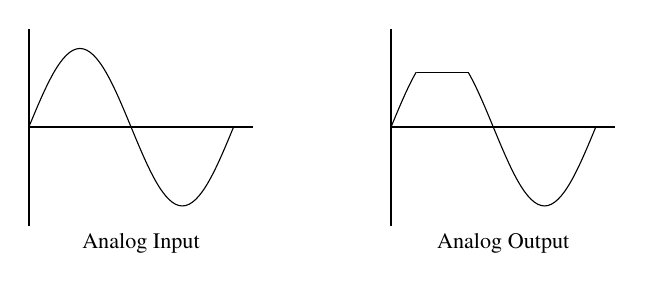
\begin{tikzpicture}
      % Coordinates
      \def\p{0.65}
      \coordinate (Origin1) at (0,0);
      \coordinate (Origin2) at (4.6,0);
      % Captions
      \draw[thick] (Origin1) -- ++(\p*4+0.25, 0)
      node[midway,below=1.2cm]{Analog Input};
      \draw[thick] (Origin2) -- ++(\p*4+0.25, 0)
      node[midway,below=1.2cm]{Analog Output};
      % Input wave
      \draw[thick] (Origin1) -- ++(0,1.25) (Origin1) -- ++(0,-1.25);
      \draw (Origin1) sin ++(\p,1) cos ++(\p,-1) sin ++(\p,-1) cos ++(\p,1);
      % Output wave
      \draw[thick] (Origin2) -- ++(0,1.25) (Origin2) -- ++(0,-1.25);
      \draw (Origin2) sin ++(\p,1) cos ++(\p,-1) sin ++(\p,-1) cos ++(\p,1);
      \draw[fill=white,draw=none]
      (Origin2) ++(\p*0.2,0.7) rectangle ++(\p*4,0.4);
      \draw (Origin2) ++(\p*0.5,0.7) -- ++(\p,0);
   \end{tikzpicture}
\end{center}
\end{center}
\end{minipage}\hspace{0.5ex}{\vrule width 1pt}\hspace{0.5ex}
\begin{minipage}[t]{0.49\linewidth}
\noindent
\begin{center}
   \begin{circuitikz}
      \draw
         (0, 0) node[op amp] (opamp) {}
         (opamp.up) -- ++(0,1)
         node[above]{$+v_{CC}$}
         (opamp.down) -- ++(0,-1)
         node[below]{$-v_{EE}$}

         (opamp.down) ++(0,-0.5) -- ++(1.25,0)
         to[R=$R_2$] ++(0,-1.5)
         node[ground]{}

         (opamp.out) ++(1.5,0) coordinate (OC)
         (opamp.out) to[diode] (OC)
         (OC) ++(-0.3,0.6)
         node[left]{$D_1$}

         (opamp.-) -- ++(-0.8,0) -- ++(0,2) coordinate (leftC) -- (leftC -| OC)
         to[short,-*] (OC) to [short,-o] ++(1,0)
         node[label=right:$V_{o}$]{}
         (opamp.+) -- ++(-0.3,0)
         to[sV, fill=white] ++(0,0) to[short,-o] ++(-0.7,0)
         node[label=left:$V_{i}$]{}
   ;
   \draw[->] (OC) to[R=$R1$] ++(0,-1.8) -- ++(-0.7,0);
   \draw[<->] (OC) ++(0,-2) -- ++(0,-1);
   \draw (OC) ++(0,-2.5) node[right]{$V_{ref}$};
\end{circuitikz}

Negative Clipper 
\begin{center}
   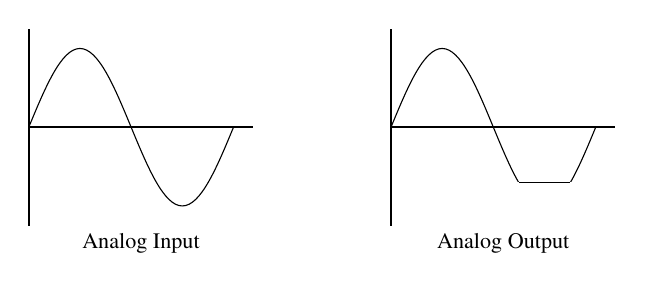
\begin{tikzpicture}
      % Coordinates
      \def\p{0.65}
      \coordinate (Origin1) at (0,0);
      \coordinate (Origin2) at (4.6,0);
      % Captions
      \draw[thick] (Origin1) -- ++(\p*4+0.25, 0)
      node[midway,below=1.2cm]{Analog Input};
      \draw[thick] (Origin2) -- ++(\p*4+0.25, 0)
      node[midway,below=1.2cm]{Analog Output};
      % Input wave
      \draw[thick] (Origin1) -- ++(0,1.25) (Origin1) -- ++(0,-1.25);
      \draw (Origin1) sin ++(\p,1) cos ++(\p,-1) sin ++(\p,-1) cos ++(\p,1);
      % Output wave
      \draw[thick] (Origin2) -- ++(0,1.25) (Origin2) -- ++(0,-1.25);
      \draw (Origin2) sin ++(\p,1) cos ++(\p,-1) sin ++(\p,-1) cos ++(\p,1);
      \draw[fill=white,draw=none]
      (Origin2) ++ (\p*0.2,-0.7) rectangle ++(\p*4,-0.4);
      \draw (Origin2) ++(\p*2.5,-0.7) -- ++(\p,0);
   \end{tikzpicture}
\end{center}
\end{center}
\end{minipage}


\CHeading{Op-Amp: \cyan{Half Wave Rectifier}}

\begin{minipage}[t]{0.49\linewidth}
\noindent
\begin{center}
   \begin{circuitikz}
      \draw
         (0, 0) node[op amp] (opamp) {}
         (opamp.up) -- ++(0,1)
         node[above]{$+v_{CC}$}
         (opamp.down) -- ++(0,-1)
         node[below]{$-v_{EE}$}

         (opamp.out) ++(1.5,0) coordinate (OC)
         (opamp.out) to[diode] (OC)
         (OC) ++(-0.3,0.6)
         node[left]{$D_1$}

         (OC) to[R=$R1$] ++(0,-1.8)
         node[ground]{}

         (opamp.-) -- ++(-0.8,0) -- ++(0,2) coordinate (leftC) -- (leftC -| OC)
         to[short,-*] (OC) to [short,-o] ++(1,0)
         node[label=right:$V_{o}$]{}
         (opamp.+) -- ++(-0.3,0)
         to[sV, fill=white] ++(0,0) to[short,-o] ++(-0.7,0)
         node[label=left:$V_{i}$]{}
   ;
\end{circuitikz}

Positive Half Wave Rectifier

\begin{center}
   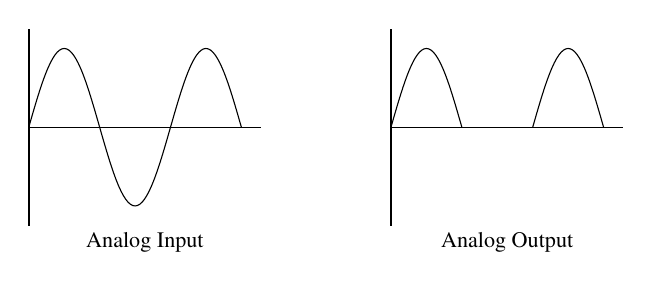
\begin{tikzpicture}
      % Coordinates
      \def\p{0.45}
      \coordinate (Origin1) at (0,0);
      \coordinate (Origin2) at (4.6,0);
      % Captions
      \draw (Origin1) -- ++(\p*6+0.25, 0)
      node[midway,below=1.2cm]{Analog Input};
      \draw (Origin2) -- ++(\p*6+0.25, 0)
      node[midway,below=1.2cm]{Analog Output};
      % Input wave
      \draw[thick] (Origin1) -- ++(0,1.25) (Origin1) -- ++(0,-1.25);
      \draw (Origin1) sin ++(\p,1) cos ++(\p,-1) sin ++(\p,-1) cos ++(\p,1) sin ++(\p,1) cos ++(\p,-1);
      % Output wave
      \draw[thick] (Origin2) -- ++(0,1.25) (Origin2) -- ++(0,-1.25);
      \draw (Origin2) sin ++(\p,1) cos ++(\p,-1) ++(\p,-1) ++(\p,1) sin ++(\p,1) cos ++(\p,-1);
   \end{tikzpicture}
\end{center}
\end{center}
\end{minipage}\hspace{0.5ex}{\vrule width 1pt}\hspace{0.5ex}
\begin{minipage}[t]{0.49\linewidth}
\noindent
\begin{center}
   \begin{circuitikz}
      \draw
         (0, 0) node[op amp] (opamp) {}
         (opamp.up) -- ++(0,1)
         node[above]{$+v_{CC}$}
         (opamp.down) -- ++(0,-1)
         node[below]{$-v_{EE}$}

         (opamp.out) ++(1.5,0) coordinate (OC)
         to[diode] (opamp.out)
         (OC) ++(-0.3,0.6)
         node[left]{$D_1$}

         (OC) to[R=$R1$] ++(0,-1.8)
         node[ground]{}

         (opamp.-) -- ++(-0.8,0) -- ++(0,2) coordinate (leftC) -- (leftC -| OC)
         to[short,-*] (OC) to [short,-o] ++(1,0)
         node[label=right:$V_{o}$]{}
         (opamp.+) -- ++(-0.3,0)
         to[sV, fill=white] ++(0,0) to[short,-o] ++(-0.7,0)
         node[label=left:$V_{i}$]{}
   ;\end{circuitikz}

Negative Half Wave Rectifier 
\begin{center}
   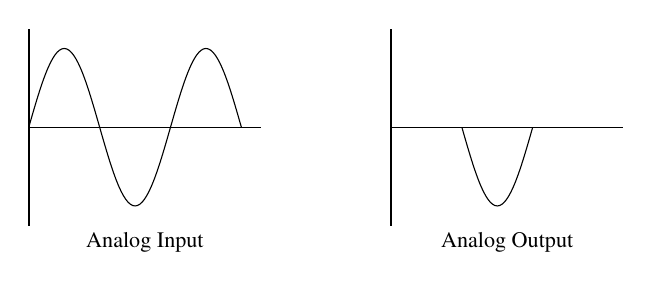
\begin{tikzpicture}
      % Coordinates
      \def\p{0.45}
      \coordinate (Origin1) at (0,0);
      \coordinate (Origin2) at (4.6,0);
      % Captions
      \draw (Origin1) -- ++(\p*6+0.25, 0)
      node[midway,below=1.2cm]{Analog Input};
      \draw (Origin2) -- ++(\p*6+0.25, 0)
      node[midway,below=1.2cm]{Analog Output};
      % Input wave
      \draw[thick] (Origin1) -- ++(0,1.25) (Origin1) -- ++(0,-1.25);
      \draw (Origin1) sin ++(\p,1) cos ++(\p,-1) sin ++(\p,-1) cos ++(\p,1) sin ++(\p,1) cos ++(\p,-1);
      % Output wave
      \draw[thick] (Origin2) -- ++(0,1.25) (Origin2) -- ++(0,-1.25);
      \draw (Origin2) ++(\p,1) ++(\p,-1) sin ++(\p,-1) cos ++(\p,1) ++(\p,1) ++(\p,-1);
   \end{tikzpicture}
\end{center}
\end{center}
\end{minipage}


\pagebreak
\vspace*{-\baselineskip}
\CHeading{Op-Amp: \cyan{Clamper Circuit}}
\begin{minipage}[t]{0.49\linewidth}
\noindent
\begin{center}
   \begin{circuitikz}
      \draw
         (0, 0) node[op amp] (opamp) {}
         (opamp.up) -- ++(0,1)
         node[above]{$+v_{CC}$}
         (opamp.down) -- ++(0,-1)
         node[below]{$-v_{EE}$}

         (opamp.down) ++(0,-0.7) -- ++(-1.25,0)
         to[R=$R_2$] ++(0,-1.3)
         node[ground]{}

         (opamp.out) ++(1.5,0) coordinate (OC)
         (opamp.out) to[diode] (OC)
         (OC) ++(-0.3,0.6)
         node[left]{$D_1$}

         (opamp.-) ++(-0.8,2) to[C] ++(-2,0)
         % to[sV, fill=white] ++(0,0) to[short,-o] ++(-0.7,0)
         node[label=left:$V_{i}$]{}

         (opamp.-) -- ++(-0.8,0) to[R=$R_1$] ++(0,2)coordinate (leftC) -- (leftC -| OC)
         to[short,-*] (OC) to [short,-o] ++(1,0)
         node[label=right:$V_{o}$]{}
   ;
   \draw[->] (opamp.+) -- ++(-1.5,0) |- ++(1,-1.3);
   \draw[<->] (opamp.+) ++(-1.5,-1.5) -- ++(0,-1);
   \draw (opamp.+) ++(-1.5,-1.9) node[left]{$V_{ref}$};
\end{circuitikz}

Positive Clamper

\begin{center}
   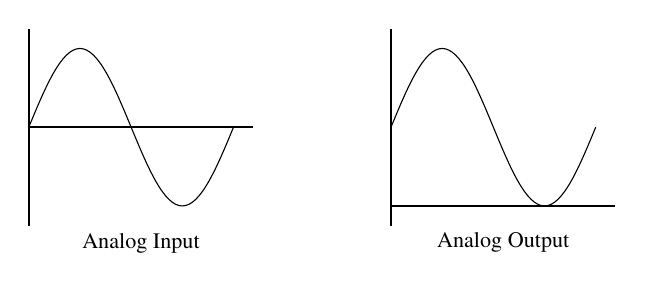
\begin{tikzpicture}
      % Coordinates
      \def\p{0.65}
      \coordinate (Axis2) at (4.6,-1);
      \coordinate (Origin1) at (0,0);
      \coordinate (Origin2) at (4.6,0);
      % Captions
      \draw[thick] (Origin1) -- ++(\p*4+0.25, 0)
      node[midway,below=1.2cm]{Analog Input};
      \draw[thick] (Axis2) -- ++(\p*4+0.25, 0);
      \draw[draw=none] (Origin2) -- ++(\p*4+0.25, 0)
      node[midway,below=1.2cm]{Analog Output};
      % Input wave
      \draw[thick] (Origin1) -- ++(0,1.25) (Origin1) -- ++(0,-1.25);
      \draw (Origin1) sin ++(\p,1) cos ++(\p,-1) sin ++(\p,-1) cos ++(\p,1);
      % Output wave
      \draw[thick] (Axis2) -- ++(0,2.25) (Axis2) -- ++(0,-0.25);
      \draw (Origin2) sin ++(\p,1) cos ++(\p,-1) sin ++(\p,-1) cos ++(\p,1);
   \end{tikzpicture}
\end{center}

\end{center}
\end{minipage}\hspace{0.5ex}{\vrule width 1pt}\hspace{0.5ex}
\begin{minipage}[t]{0.49\linewidth}
\noindent
\begin{center}
   \begin{circuitikz}
      \draw
         (0, 0) node[op amp] (opamp) {}
         (opamp.up) -- ++(0,1)
         node[above]{$+v_{CC}$}
         (opamp.down) -- ++(0,-1)
         node[below]{$-v_{EE}$}

         (opamp.down) ++(0,-0.7) -- ++(-1.25,0)
         to[R=$R_2$] ++(0,-1.3)
         node[ground]{}

         (opamp.out) ++(1.5,0) coordinate (OC)
         (opamp.out) to[diode] (OC)
         (OC) ++(-0.3,0.6)
         node[left]{$D_1$}

         (opamp.-) ++(-0.8,2) to[C] ++(-2,0)
         node[label=left:$V_{i}$]{}

         (opamp.-) -- ++(-0.8,0) to[R=$R_1$] ++(0,2)coordinate (leftC) -- (leftC -| OC)
         to[short,-*] (OC) to [short,-o] ++(1,0)
         node[label=right:$V_{o}$]{}
   ;
   \draw[->] (opamp.+) -- ++(-1.5,0) |- ++(1,-1.3);
   \draw[<->] (opamp.+) ++(-1.5,-1.5) -- ++(0,-1);
   \draw (opamp.+) ++(-1.5,-1.9) node[left]{$V_{ref}$};
\end{circuitikz}

Negative Clamper

\begin{center}
   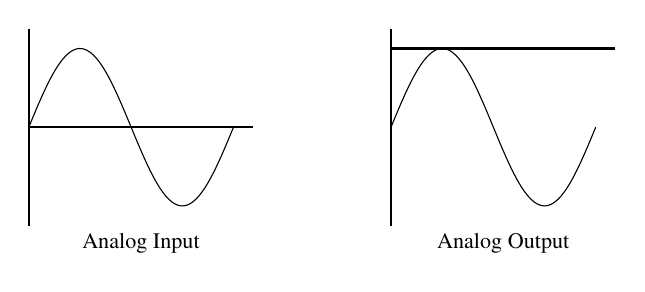
\begin{tikzpicture}
      % Coordinates
      \def\p{0.65}
      \coordinate (Origin1) at (0,0);
      \coordinate (Origin2) at (4.6,0);
      \coordinate (Axis2) at (4.6,1);
      % Captions
      \draw[thick] (Origin1) -- ++(\p*4+0.25, 0)
      node[midway,below=1.2cm]{Analog Input};
      \draw[thick] (Axis2) -- ++(\p*4+0.25, 0)
      node[midway,below=2.2cm]{Analog Output};
      % Input wave
      \draw[thick] (Origin1) -- ++(0,1.25) (Origin1) -- ++(0,-1.25);
      \draw (Origin1) sin ++(\p,1) cos ++(\p,-1) sin ++(\p,-1) cos ++(\p,1);
      % Output wave
      \draw[thick] (Origin2) -- ++(0,1.25) (Origin2) -- ++(0,-1.25);
      \draw (Origin2) sin ++(\p,1) cos ++(\p,-1) sin ++(\p,-1) cos ++(\p,1);
   \end{tikzpicture}
\end{center}
\end{center}
\end{minipage}


\CHeading{Op-Amp: \cyan{Common Mode}}
When two input signals voltages of same phase, frequency and magnitude are applied are applied to both inputs, they tend to cancel each other resulting in a zero-output voltage. This action is called common mode rejection.

\begin{center}
   \begin{circuitikz}
      \draw
      (0, 0) node[op amp] (opamp) {}
      (opamp.-) to[short,-o] ++(-0.5,0) node[left]{$v_1$}
      (opamp.+) to[short,-o] ++(-0.5,0) node[left]{$v_2$}
      (opamp.out) to[short,-o] ++(0.5,0) node[right]{$0v$}
   ;\end{circuitikz}
\end{center}

\Heading{Common Mode Rejection Ratio (CMRR)}
Unwanted signals or noise appearing with same polarity on
both lines of input are common mode signals and are
cancelled by the op-amp. The measure of the op-amp's
ability to reject common mode signals is expressed in terms of
common mode rejection ratio (CMRR). It is defined as

\vspace{-0.5\baselineskip}
$$CMRR = \frac{A_d}{A_c}$$

\Heading{Maximum Output Voltage Swing}
   The output voltage never excess the DC voltage supply $($-$v$ \ to \ +$v)$ of the Op-Amp.

\pagebreak
\Title{Flash ADC: \cyan{3 bit}}
\textbf{Components of Flash ADC}: Structure of Flash ADC consist three major components --

\vspace{-0.5\baselineskip}
\begin{enumerate}
\item High Speed Comparator $[2^n - 1]$
\item Resistive voltage divider Network $[2^n]$
\item Priority Encoder $[1]$
\end{enumerate}

\begin{center}
   \begin{circuitikz}
      \draw
      (0, 12) node[op amp, scale=0.8] (opamp7) {}
      (0, 10) node[op amp, scale=0.8] (opamp6) {}
      (0, 8) node[op amp, scale=0.8] (opamp5) {}
      (0, 6) node[op amp, scale=0.8] (opamp4) {}
      (0, 4) node[op amp, scale=0.8] (opamp3) {}
      (0, 2) node[op amp, scale=0.8] (opamp2) {}
      (0, 0) node[op amp, scale=0.8] (opamp1) {}

      (opamp7.out) node[right]{$7$}
      (opamp6.out) node[right]{$6$}
      (opamp5.out) node[right]{$5$}
      (opamp4.out) node[right]{$4$}
      (opamp3.out) node[right]{$3$}
      (opamp2.out) node[right]{$2$}
      (opamp1.out) node[right]{$1$}

      (opamp7.-) to[crossing] ++(-1,0) to[short,-*] ++(-1,0)
      node[left]{$\frac{7}{8}V_{ref} \tabs V_{7}$}
      (opamp6.-) to[crossing] ++(-1,0) to[short,-*] ++(-1,0)
      node[left]{$\frac{6}{8}V_{ref} \tabs V_{6}$}
      (opamp5.-) to[crossing] ++(-1,0) to[short,-*] ++(-1,0)
      node[left]{$\frac{5}{8}V_{ref} \tabs V_{5}$}
      (opamp4.-) to[crossing] ++(-1,0) to[short,-*] ++(-1,0)
      node[left]{$\frac{4}{8}V_{ref} \tabs V_{4}$}
      (opamp3.-) to[crossing] ++(-1,0) to[short,-*] ++(-1,0)
      node[left]{$\frac{3}{8}V_{ref} \tabs V_{3}$}
      (opamp2.-) to[crossing] ++(-1,0) to[short,-*] ++(-1,0)
      node[left]{$\frac{2}{8}V_{ref} \tabs V_{2}$}
      (opamp1.-) to[short,-*] ++(-2,0)
      node[left]{$\frac{1}{8}V_{ref} \tabs V_{1}$}

      (opamp7.-) ++(-2,0) coordinate (7P) ++(0,2) to[R,l=$R_8$] ++(0,-2)
      
      (7P) to[R,l=$R_7$] ++(0,-2) to[R,l=$R_6$] ++(0,-2) to[R,l=$R_5$] ++(0,-2) to[R,l=$R_4$] ++(0,-2) to[R,l=$R_3$] ++(0,-2) to[R,l=$R_2$] ++(0,-2) to[R,l=$R_1$] ++(0,-2)
      node[ground]{}

      (7P) ++(0,2) node[above]{$V_{ref}$}

      (opamp1.+) to[short,-*] ++(-0.5,0)
      -- ++(0,14) node[above]{$V_{in}$}

      (opamp7.+) to[short,-*] ++(-0.5,0)
      (opamp6.+) to[short,-*] ++(-0.5,0)
      (opamp5.+) to[short,-*] ++(-0.5,0)
      (opamp4.+) to[short,-*] ++(-0.5,0)
      (opamp3.+) to[short,-*] ++(-0.5,0)
      (opamp2.+) to[short,-*] ++(-0.5,0)
      
      (3.5, 7) -- ++(1.5,0) node[right]{$C$}
      (3.5, 6) -- ++(1.5,0) node[right]{$B$}
      (3.5, 5) -- ++(1.5,0) node[right]{$A$}
      
      (3.7,7) node[above right]{$MSB$}
      (3.7,5) node[below right]{$LSB$}
      (2.25,-1.5) -- ++(0,-0.4) node[ground]{}
      (1,-1) -- ++(-0.5,0) |- (2.25,-1.9)
      (2.25,-1.9) to[short,-*] (2.25,-1.9)
      (1,-1)  node[right]{$0$}

      [fill=white](1,-1.5) rectangle (3.5,12.5)
      node[pos=.5, align=center] {Priority \\[-1ex] Encoder}
      ;
   \end{circuitikz}
\end{center}

\pagebreak
\vspace*{-\baselineskip}
\CHeading{Op-Amp: \cyan{Extra Terms}}
\textbf{Input Offset Voltage}: The input offset voltage $(V_{iO})$ is defined as the voltage that must be applied between the two input terminals of the op amp to obtain zero volts at the output.

\vspace{2ex}
\textbf{Input Bias Current}: Ideally no current flows into the input terminals of op-amp. But in practice, a small amount of current flows into the input terminals. These currents are called bias current.

\vspace{2ex}
\textbf{Input Offset Current}: The difference between these two input bias currents are called input offset current.

\vspace{2ex}
\textbf{Input Impedance}: The input impedance in the differential mode is the total resistance between inverting and noninverting inputs.

\vspace{2ex}
\textbf{Output Impedance}: The output impedance is the resistance viewed from the output terminal of the op-amp.

\vspace{2ex}
\textbf{Slew rate}: The slew rate is defined as the maximum rate of output voltage change per unit time.
\vspace{-0.5\baselineskip}
$$\text{Slew rate} = \frac{\Delta V_{out}}{\Delta t}$$
\end{document}